\section{Soll-Ist-Zeit-Vergleich}

\begin{table}[H]
    \begin{tabular}{|p{5cm}|p{2cm}|p{2cm}|p{2cm}|}
    \hline    
    \rowcolor{lightblue}
	Phase & Soll & Ist & Differenz \\ \hline
	Inception & 36.00 &	45.50 &	-9.50 \\ \hline
	Elaboration1 & 111.00 & 150.50	& -39.50 \\ \hline
	Elaboration2 & 98.00 & 105.75 & -7.75 \\ \hline
	Construction1 & 110.00 & 122.50 & -12.50 \\ \hline
	\rowcolor{lightblue}
	Total & & & \\ \hline
    \end{tabular}
    \caption[Phasen]{Phasen}
\end{table}

\subsection{Inception}
\begin{tabbing}[H]
    \hspace*{6cm}\=\hspace*{6cm}\= \kill
    Start: \> 14.09.2015 \\
	Ende: \> 23.09.2015 \\
\end{tabbing}
\begin{figure}[H]
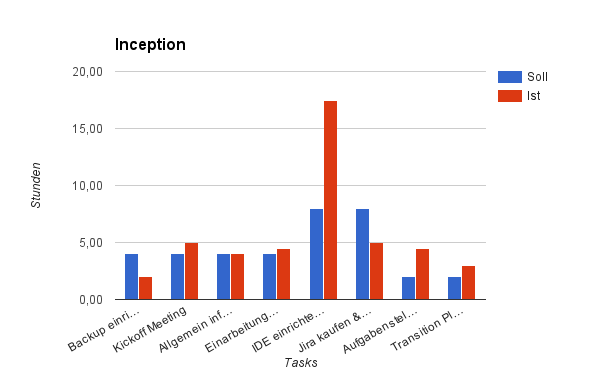
\includegraphics[width=\textwidth]{images/inception.png}
\caption[Inception]{Inception}
\end{figure}

\subsection{Elaboration1}
\begin{tabbing}[H]
    \hspace*{6cm}\=\hspace*{6cm}\= \kill
    Start: \> 23.09.2015 \\
	Ende: \> 19.10.2015 \\
\end{tabbing}
\begin{figure}[H]
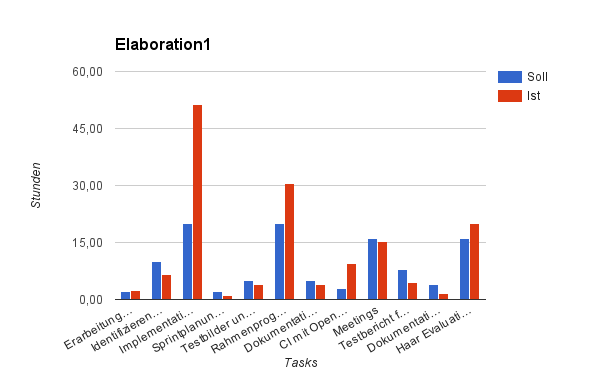
\includegraphics[width=\textwidth]{images/elab1.png}
\caption[Elaboration1]{Elaboration1}
\end{figure}

\subsection{Elaboration2}
\begin{tabbing}[H]
    \hspace*{6cm}\=\hspace*{6cm}\= \kill
    Start: \> 19.10.2015 \\
	Ende: \>  04.11.2015 \\
\end{tabbing}
\begin{figure}[H]
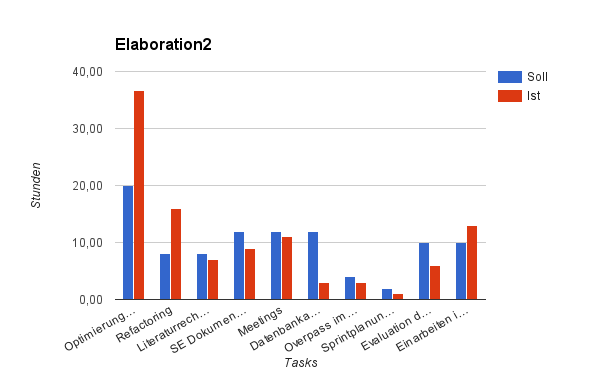
\includegraphics[width=\textwidth]{images/elab2.png}
\caption[Elaboration2]{Elaboration2}
\end{figure}

\subsection{Construction1}
\begin{tabbing}[H]
    \hspace*{6cm}\=\hspace*{6cm}\= \kill
    Start: \> 04.11.2015 \\
	Ende: \>  25.11.2015 \\
\end{tabbing}
\begin{figure}[H]
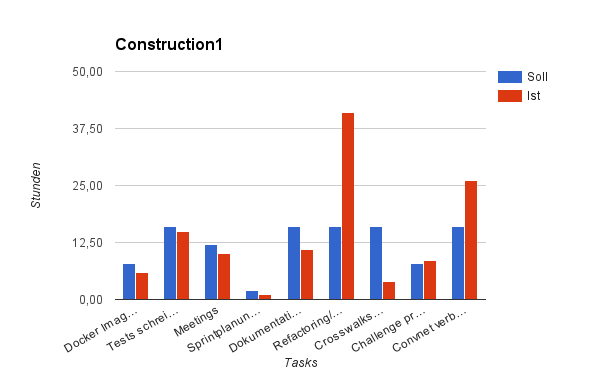
\includegraphics[width=\textwidth]{images/construction1.png}
\caption[Construction1]{Construction1}
\end{figure}

\subsection{Construction2}
\begin{tabbing}[H]
    \hspace*{6cm}\=\hspace*{6cm}\= \kill
    Start: \> 04.11.2015 \\
	Ende: \>  11.11.2015 \\
\end{tabbing}

\subsection{Transition}
\begin{tabbing}[H]
    \hspace*{6cm}\=\hspace*{6cm}\= \kill
    Start: \> 11.11.2015 \\
	Ende: \>  18.11.2015 \\
\end{tabbing}
